\begin{figure}[htbp]
\centering
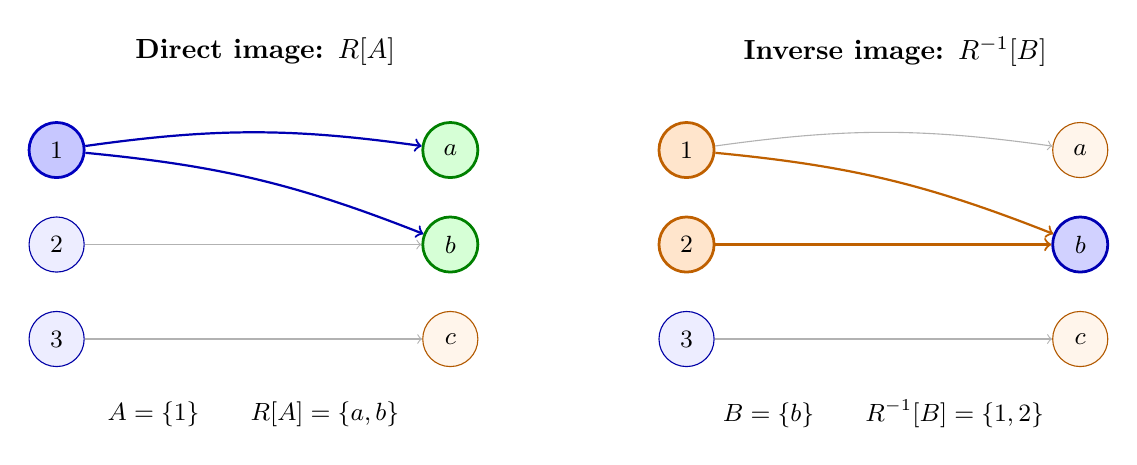
\begin{tikzpicture}[x=1cm,y=1cm,font=\small,source/.style={circle,draw=blue!65!black,fill=blue!7,minimum size=0.7cm},target/.style={circle,draw=orange!70!black,fill=orange!8,minimum size=0.7cm}]
    \node[font=\bfseries] at (3.55,4.25) {Direct image: $R[A]$};
    \node[font=\bfseries] at (11.55,4.25) {Inverse image: $R^{-1}[B]$};
    \begin{scope}
        \node[source,fill=blue!22,draw=blue!75!black,line width=1pt] (x1) at (0.9,3) {$1$};
        \node[source] (x2) at (0.9,1.8) {$2$};
        \node[source] (x3) at (0.9,0.6) {$3$};
        \node[target,fill=green!16,draw=green!50!black,line width=1pt] (a) at (5.9,3) {$a$};
        \node[target,fill=green!16,draw=green!50!black,line width=1pt] (b) at (5.9,1.8) {$b$};
        \node[target] (c) at (5.9,0.6) {$c$};
        \draw[->,thick,blue!70!black] (x1) to[bend left=8] (a);
        \draw[->,thick,blue!70!black] (x1) to[bend left=8] (b);
        \draw[->,gray!60] (x2) -- (b);
        \draw[->,gray!60] (x3) -- (c);
        \node[align=center,font=\small] at (3.4,-0.35) {$A=\{1\}$\qquad $R[A]=\{a,b\}$};
    \end{scope}
    \begin{scope}[xshift=8cm]
        \node[source,fill=orange!20,draw=orange!75!black,line width=1pt] (u1) at (0.9,3) {$1$};
        \node[source,fill=orange!20,draw=orange!75!black,line width=1pt] (u2) at (0.9,1.8) {$2$};
        \node[source] (u3) at (0.9,0.6) {$3$};
        \node[target] (v1) at (5.9,3) {$a$};
        \node[target,fill=blue!18,draw=blue!70!black,line width=1pt] (v2) at (5.9,1.8) {$b$};
        \node[target] (v3) at (5.9,0.6) {$c$};
        \draw[->,gray!60] (u1) to[bend left=8] (v1);
        \draw[->,thick,orange!75!black] (u1) to[bend left=8] (v2);
        \draw[->,thick,orange!75!black] (u2) -- (v2);
        \draw[->,gray!60] (u3) -- (v3);
        \node[align=center,font=\small] at (3.4,-0.35) {$B=\{b\}$\qquad $R^{-1}[B]=\{1,2\}$};
    \end{scope}
\end{tikzpicture}
\caption{For the same relation, the direct image collects targets reached from $A$, while the inverse image collects sources that reach $B$.}
\label{fig:relation-images}
\end{figure}